\section{Tensor Network Simulation}
tensors are mathematical objects have a lot in common with nd-arrays, some examples of tensors you are probably familliar with, a rank 0 tensor is just a scalar, a rank 1 tensor is a vector, a rank 2 tensor is a matrix, and so on. The rank of the tensor tells you how many indecies you need to describe a single element in the tensor, e.g. you need 1 index to tell which element in a vector you are talking about and you need 2, namely a column and row index to uniquely specify an element in a matrix. 
Each index has a dimension, for example a rank 2 tensor that is m by n would have one index $i$ taking one of n values and another index $j$ taking one of m values, typically $i\in \{0,1,..,n-1\}, j\in \{0,1,..,m-1\}$, we can then describe an element by $a_{ij}$, if we have more indecies they are sometimes written as $a_{ij}^{kl}$.
\begin{figure}[H]
    \centering 
    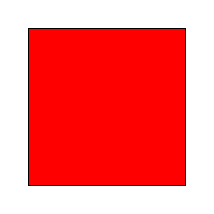
\begin{tikzpicture}
        \draw[fill=red] (0,0) rectangle (2,2) node[pos=0.5]{};
    \end{tikzpicture}
    \caption{rank 0 tensor.}
    \label{fig:r0t}
\end{figure}

\begin{figure}[H]
    \centering 
    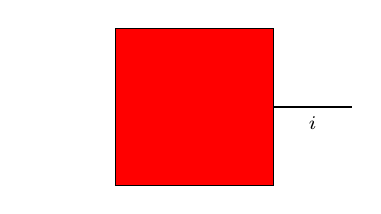
\begin{tikzpicture}
        \draw[fill=red] (0,0) rectangle (2,2) node[pos=0.5]{};
        \draw[](2, 1) -- (3, 1) 
         node[draw=none,fill=none,font=\scriptsize,midway,below]{$i$};
        \draw (-1, 1) node[draw=none]{};
    \end{tikzpicture}
    \caption{rank 1 tensor. Each index is repressented by a line}
    \label{fig:r1t}
\end{figure}

\begin{figure}[H]
    \centering 
    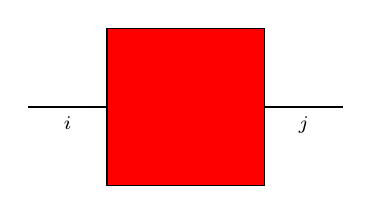
\begin{tikzpicture}
        \draw[fill=red] (0,0) rectangle (2,2) node[pos=0.5]{};
        \draw[](2, 1) -- (3, 1)  
         node[draw=none,fill=none,font=\scriptsize,midway,below]{$j$};
        \draw[](0, 1) -- (-1, 1)  
         node[draw=none,fill=none,font=\scriptsize,midway,below]{$i$};
        
    \end{tikzpicture}
    \caption{rank 2 tensor. Each index is repressented by a line}
    \label{fig:r2t}
\end{figure}

\noindent
Often the indecies are not numbered on these drawing. If we have two tensors we can make them share an index if they have the same dimension, so if we have two rank 3 tensors, one where we have the dimensions of the indexes be 2, 3, 5 and another where it is 1, 4, 3. We can see that they both have an index of size 3 so if we wish we can make them share label for this index. Thus they could have the indecies i, j, k and l, m, j, notice the reuse of j. 

\begin{figure}[H]
    \centering 
    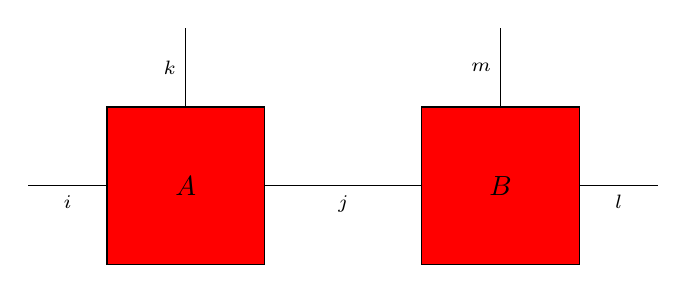
\begin{tikzpicture}
        \draw[fill=red] (0,0) rectangle (2,2) node[pos=0.5]{$A$};
        \draw[](2, 1) -- (3, 1)  
         node[draw=none,fill=none,font=\scriptsize,midway,below]{};
        \draw[](0, 1) -- (-1, 1)  
         node[draw=none,fill=none,font=\scriptsize,midway,below]{$i$};
        \draw[](1, 2) -- (1, 3)  
         node[draw=none,fill=none,font=\scriptsize,midway,left]{$k$};
        
        \draw[fill=red](4,0) rectangle (6,2) node[pos=0.5]{$B$};
        \draw[](6, 1) -- (7, 1)  
         node[draw=none,fill=none,font=\scriptsize,midway,below]{$l$};
        \draw[](4, 1) -- (3, 1)  
         node[draw=none,fill=none,font=\scriptsize,below]{$j$};
        \draw[](5, 2) -- (5, 3)  
         node[draw=none,fill=none,font=\scriptsize,midway,left]{$m$};
    \end{tikzpicture}
    \caption{rank 3 tensors sharing index $j$.}
    \label{fig:2r3t}
\end{figure}

\noindent
But what is this good for? In essence, when we make tensors share indecies it is a way to symbolise that we are multiplying them, matrix multiplication style. The acctual computation of the multiplication can be done at a later point we are just marking our intention. This is important as we might want to build an entire network of tensors and then be strategic about which shared indecies we choose to \textit{contract}. Contracting a shared index is synonumus with computing the product of the two tensors. 
\begin{figure}[H]
    \centering 
    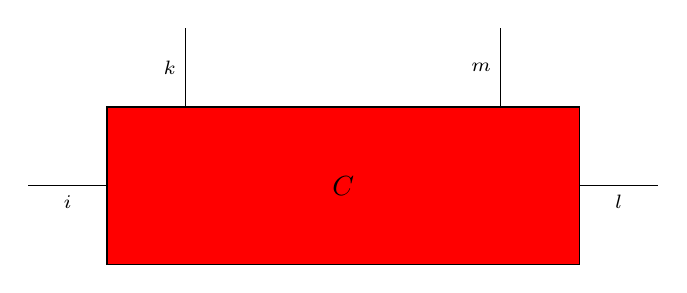
\begin{tikzpicture}
        \draw[fill=red](0,0) rectangle (6,2) node[pos=0.5]{$C$};
        \draw[](0, 1) -- (-1, 1)  
         node[draw=none,fill=none,font=\scriptsize,midway,below]{$i$};
        \draw[](1, 2) -- (1, 3)  
         node[draw=none,fill=none,font=\scriptsize,midway,left]{$k$};
        
        \draw[](6, 1) -- (7, 1)  
         node[draw=none,fill=none,font=\scriptsize,midway,below]{$l$};
        \draw[](5, 2) -- (5, 3)  
         node[draw=none,fill=none,font=\scriptsize,midway,left]{$m$};
    \end{tikzpicture}
    \caption{rank 4 tensor after contracting shared index $j$ from Figure \ref{fig:2r3t}.}
    \label{fig:4t}
\end{figure}
\noindent
in this example we have two tensors A and B where each have elements of the form $a_{ijk}, b_{lmj}$ resulting in a single tensor C with the elements $$c_{iklm}=\displaystyle\sum_{x=0}^{dim(j)-1} a_{ixk}b_{lmx} $$
here $dim(j)=3$ and we subtract 1 since the elements are 0 indexed. In \textit{tensor notation} the summation is implicit if there is a shared index in such an equation so we would just write $c_{iklm}=a_{ijk}b_{lmj}$

\noindent
We can use a tensor network to represent our $QFT$ cirquit and our state. We will use a matrix product state (MPS) to represent our state, and a matrix product operator (MPO) to repressent our circuit, these are just sub categories of tensor networks. 

\begin{figure}[H]
    \centering 
    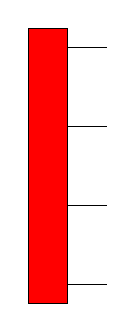
\begin{tikzpicture}
        \draw[] (0.25,-1) -- (0.25,-4);
        \foreach \i in {1,...,4}
        {
                \draw[](0.5, -\i +0.25) -- (1, -\i +0.25); 
        }
        \draw[fill=red] (0,-0.5) rectangle (0.5,-4) node[pos=0.5]{};
    \end{tikzpicture}
    \caption{4 qubit state repressented as a tensor. (MPS)}
    \label{fig:psi4t}
\end{figure}
\noindent
Here we have the whole state in one large tensor. This is highly undesirable as this uses a lot of memory, we would rather construct a network of tensors. Let us take the state $\ket{0010}$ as an example.
%TODO: explain SVD and why we use swap gates. 
\begin{figure}[H]
    \centering 
    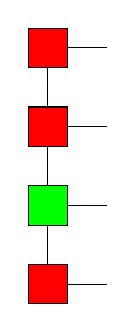
\begin{tikzpicture}
        \draw[] (0.25,-1) -- (0.25,-4);
        \foreach \i in {1,...,4}
        {
                \draw[](0.5, -\i +0.25) -- (1, -\i +0.25); 
                \draw[fill=red] (0,-\i) rectangle (0.5,-\i+0.5) node[pos=0.5]{};
        }
        \draw[fill=green] (0,-3) rectangle (0.5,-3+0.5) node[pos=0.5]{};
    \end{tikzpicture}
    \caption{4 qubit state $\ket{0010}$ repressented as a tensor network (MPS). Red represents $\ket{0}$ and green $\ket{1}$. }
    \label{fig:psi4t_mps}
\end{figure}
\noindent 
you may remember that $\ket{\Psi}$ is a vector, in other words a rank 1 tensor, but here we are using them as rank 2 and 3 tensors, how can we do so? We can simply add some dimensions like so:
$\ket{\Psi} \rightarrow
\begin{bmatrix}
    \ket{\Psi}
\end{bmatrix} \rightarrow
\begin{bmatrix}
    \begin{bmatrix}
        \ket{\Psi}
    \end{bmatrix}
\end{bmatrix}$

\begin{figure}[H]
    \centering 
    \scalebox{0.57}{
    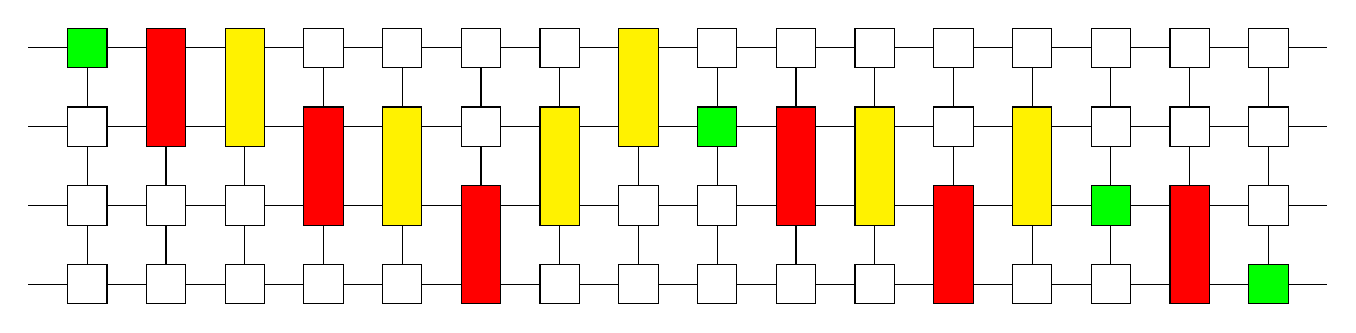
\begin{tikzpicture}
        \foreach \j in {0,...,15}{
            \draw[](\j+0.25,0) -- (\j+0.25, -3);
        }
        \foreach \i in {0,...,3}
        {
            \draw[](-0.5,-0.25-\i) -- (16, -0.25-\i);
            \foreach \j in {0,...,15}{
                \draw[fill=white] (\j,-\i) rectangle (0.5+\j,-0.5-\i) node[pos=0.5]{};
            }
        }

        \draw[fill=green] (0,0) rectangle (0.5,-0.5) node[pos=0.5]{};
        \foreach \i in {0,...,1}
        {
            \draw[fill=red] (1+\i+\i,-\i) rectangle (0.5+1+\i+\i,-0.5-1-\i) node[pos=0.5]{};
            \draw[fill=yellow] (2+\i+\i,-\i) rectangle (0.5+2+\i+\i,-0.5-1-\i) node[pos=0.5]{};
        }
        \draw[fill=red] (5,-2) rectangle (0.5+1+4,-0.5-1-2) node[pos=0.5]{};
        \draw[fill=yellow] (6,-1) rectangle (0.5+2+4,-0.5-1-1) node[pos=0.5]{};
        \draw[fill=yellow] (7,0) rectangle (0.5+2+5,-0.5-1) node[pos=0.5]{};

        \draw[fill=green] (8,-1) rectangle (0.5+8,-0.5-1) node[pos=0.5]{};
        \draw[fill=red] (9,-1) rectangle (0.5+9,-0.5-1-1) node[pos=0.5]{};
        \draw[fill=yellow] (10,-1) rectangle (0.5+10,-0.5-1-1) node[pos=0.5]{};
        \draw[fill=red] (11,-2) rectangle (0.5+11,-0.5-1-2) node[pos=0.5]{};
        \draw[fill=yellow] (12,-1) rectangle (0.5+12,-0.5-1-1) node[pos=0.5]{};

        \draw[fill=green] (13,-2) rectangle (0.5+13,-0.5-2) node[pos=0.5]{};
        \draw[fill=red] (14,-2) rectangle (0.5+14,-0.5-1-2) node[pos=0.5]{};

        \draw[fill=green] (15,-3) rectangle (0.5+15,-0.5-3) node[pos=0.5]{};
    \end{tikzpicture}
    }
    \caption{$QFT_4$ repressented as a tensor network (MPO). White repressents an identity gate, green a Hadamard gate, red a controlled $R_x,x\in \{2,3,4\}$ gate, and yellow a swap gate.}
    \label{fig:qft4t}
\end{figure}
\begin{figure}[H]
    \centering 
    \scalebox{0.57}{
    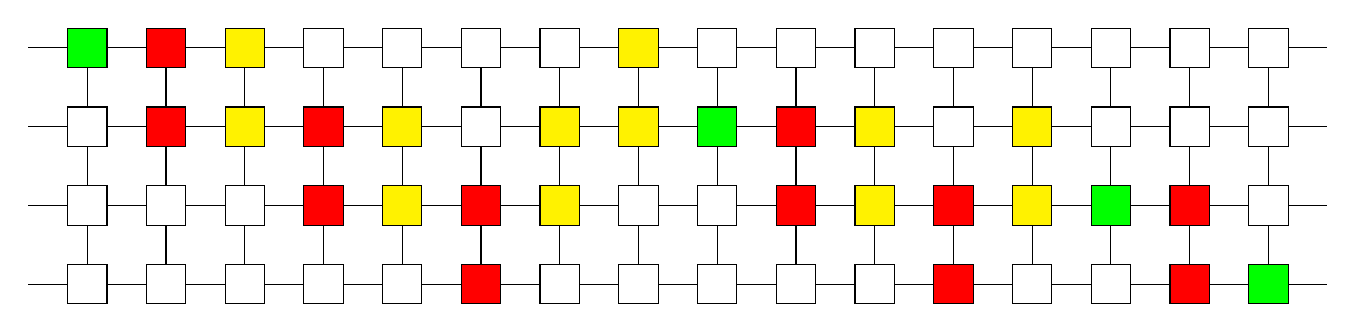
\begin{tikzpicture}
        \foreach \j in {0,...,15}{
            \draw[](\j+0.25,0) -- (\j+0.25, -3);
        }
        \foreach \i in {0,...,3}
        {
            \draw[](-0.5,-0.25-\i) -- (16, -0.25-\i);
            \foreach \j in {0,...,15}{
                \draw[fill=white] (\j,-\i) rectangle (0.5+\j,-0.5-\i) node[pos=0.5]{};
            }
        }

        \draw[fill=green] (0,0) rectangle (0.5,-0.5) node[pos=0.5]{};
        \foreach \i in {0,...,1}
        {
            \draw[fill=red] (1+\i+\i,-\i) rectangle (0.5+1+\i+\i,-0.5-\i) node[pos=0.5]{};
            \draw[fill=red] (1+\i+\i,-\i-1) rectangle (0.5+1+\i+\i,-0.5-1-\i) node[pos=0.5]{};
            \draw[fill=yellow] (2+\i+\i,-\i) rectangle (0.5+2+\i+\i,-0.5-\i) node[pos=0.5]{};
            \draw[fill=yellow] (2+\i+\i,-\i-1) rectangle (0.5+2+\i+\i,-0.5-1-\i) node[pos=0.5]{};
        }
        \draw[fill=red] (5,-2) rectangle (0.5+1+4,-0.5-2) node[pos=0.5]{};
        \draw[fill=red] (5,-3) rectangle (0.5+1+4,-0.5-1-2) node[pos=0.5]{};
        \draw[fill=yellow] (6,-1) rectangle (0.5+2+4,-0.5-1) node[pos=0.5]{};
        \draw[fill=yellow] (6,-2) rectangle (0.5+2+4,-0.5-1-1) node[pos=0.5]{};
        \draw[fill=yellow] (7,0) rectangle (0.5+2+5,-0.5) node[pos=0.5]{};
        \draw[fill=yellow] (7,-1) rectangle (0.5+2+5,-0.5-1) node[pos=0.5]{};

        \draw[fill=green] (8,-1) rectangle (0.5+8,-0.5-1) node[pos=0.5]{};
        \draw[fill=red] (9,-1) rectangle (0.5+9,-0.5-1) node[pos=0.5]{};
        \draw[fill=red] (9,-2) rectangle (0.5+9,-0.5-1-1) node[pos=0.5]{};
        \draw[fill=yellow] (10,-1) rectangle (0.5+10,-0.5-1) node[pos=0.5]{};
        \draw[fill=yellow] (10,-2) rectangle (0.5+10,-0.5-1-1) node[pos=0.5]{};
        \draw[fill=red] (11,-2) rectangle (0.5+11,-0.5-2) node[pos=0.5]{};
        \draw[fill=red] (11,-3) rectangle (0.5+11,-0.5-1-2) node[pos=0.5]{};
        \draw[fill=yellow] (12,-1) rectangle (0.5+12,-0.5-1) node[pos=0.5]{};
        \draw[fill=yellow] (12,-2) rectangle (0.5+12,-0.5-1-1) node[pos=0.5]{};

        \draw[fill=green] (13,-2) rectangle (0.5+13,-0.5-2) node[pos=0.5]{};
        \draw[fill=red] (14,-2) rectangle (0.5+14,-0.5-2) node[pos=0.5]{};
        \draw[fill=red] (14,-3) rectangle (0.5+14,-0.5-1-2) node[pos=0.5]{};

        \draw[fill=green] (15,-3) rectangle (0.5+15,-0.5-3) node[pos=0.5]{};
    \end{tikzpicture}
    }
    \caption{$QFT_4$ from figure \ref{fig:qft4t} with all two qubit gates split using SVD.}
    \label{fig:qft4t_svd}
\end{figure}

\begin{figure}[H]
    \centering 
    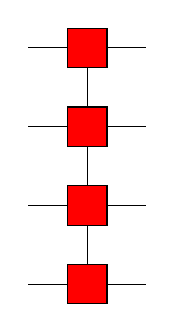
\begin{tikzpicture}
        \draw[] (0.25,-1) -- (0.25,-4);
        \foreach \i in {1,...,4}
        {
                \draw[](-0.5, -\i +0.25) -- (1, -\i +0.25); 
                \draw[fill=red] (0,-\i) rectangle (0.5,-\i+0.5) node[pos=0.5]{};
        }
    \end{tikzpicture}
    \caption{$QFT_4$ from figure \ref{fig:qft4t_svd} with 'horisontal' shared indecies contracted.}
    \label{fig:mpo}
\end{figure}
\noindent
Now that we have our state MPS and our QFT MPO we can apply the MPO to the MPS by connecting the outputs from the MPS to the inputs to the MPO and contracting those shared indexes. This results in an updated MPS. If we wish to combine two MPOs into one we do the same, just connecting the output of one to the input of another and contracting. 

\begin{figure}[H]
    \centering 
    \begin{subfigure}{.3\textwidth}
        \centering
        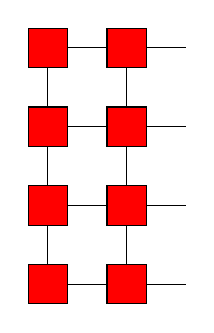
\begin{tikzpicture}
            \draw[] (0.25,-1) -- (0.25,-4);
            \draw[] (-0.75,-1) -- (-0.75,-4);
            \foreach \i in {1,...,4}
            {
                    \draw[](-0.5, -\i +0.25) -- (1, -\i +0.25); 
                    \draw[fill=red] (0,-\i) rectangle (0.5,-\i+0.5) node[pos=0.5]{};
                    \draw[fill=red] (-1,-\i) rectangle (-0.5,-\i+0.5) node[pos=0.5]{};
            }
        \end{tikzpicture}
        \caption{Before contraction.}
    \end{subfigure}%
    \begin{subfigure}{.2\textwidth}
      \centering
        $\iff$
        \vspace{5em}
    \end{subfigure}
    \begin{subfigure}{.3\textwidth}
        \hspace{2em}
        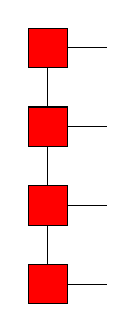
\begin{tikzpicture}
            \draw[] (0.25,-1) -- (0.25,-4);
            \foreach \i in {1,...,4}
            {
                    \draw[](0.5, -\i +0.25) -- (1, -\i +0.25); 
                    \draw[fill=red] (0,-\i) rectangle (0.5,-\i+0.5) node[pos=0.5]{};
            }
        \end{tikzpicture}
        \caption{After contraction.}
    \end{subfigure}%
    \caption{MPO applied to MPS.}
    \label{fig:mpo_mps}
\end{figure}

Now you might ask why we suddenly are using a ton of swap gates, and what are they even. Swap gates simply swap the values of two qubits, so if $\ket{10}$ goes in $\ket{01}$ commes out. This is simulated with this matrix, when swapping adjacent qubits as we are. 
\begin{figure}[H]
    \centering
    $$
    \begin{bmatrix}
        1 & 0 & 0 & 0\\ 
        0 & 0 & 1 & 0\\ 
        0 & 1 & 0 & 0\\ 
        0 & 0 & 0 & 1\\ 
    \end{bmatrix}
    $$
    \caption{SWAP gate matrix. }
    \label{fig:swap}
\end{figure}

\noindent
We do this to avoid having non-local gates in the circuit, such as the controlled $R_x$ gates we use in the QFT. This was not a concern when doing the dense simulation, but here we have to split everything up into tensors acting on individual qubits and therefor would like smaller gates to start with. The reason we have to split everything up is mostly a limitation of the liberary we are using for the simulation, it is a perfectly vallid tensor network even without splitting every gate. It does add a cost of slightly less than two swap gates per non-local gate. 
This low overhead is not something that can be achieved in general, the most general way to make every gate local requres swapping the two qubits with the ones between them until they are adjacent, applying the gate, and then swapping them back to where they came from, this takes swapgates equal to the number of qubits between the two target qubits times two. We are fortunatly in a situation where we can do this in a smarter way. 

After splitting a gate which acts on more than one qubit the index they share will have a dimension larger than 1, and when we contract a MPO like so: 
\begin{figure}[H]
    \centering 
    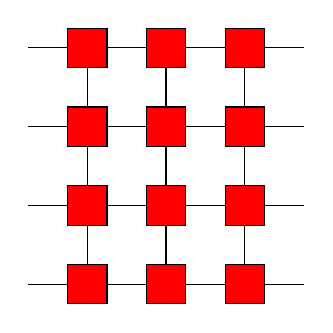
\begin{tikzpicture}
        \foreach \j in {0,...,2}
        {
            \draw[] (0.25+\j,-1) -- (0.25+\j,-4);
            \foreach \i in {1,...,4}
            {
                    \draw[](-0.5+\j, -\i +0.25) -- (1+\j, -\i +0.25); 
                    \draw[fill=red] (0+\j,-\i) rectangle (0.5+\j,-\i+0.5) node[pos=0.5]{};
            }
        }
    \end{tikzpicture}

    \caption{$QFT_4$ from figure \ref{fig:qft4t_svd} with 'horisontal' shared indecies contracted.}
    \label{fig:mpo_contraction}
\end{figure}
